\chapter{Prime Numbers on the Helix}\label{ch:primes}

This chapter shows how the conical helix provides a natural geometric
embedding of the congruence classes $n \equiv 1,5\pmod{6}$. Since all
primes $p > 3$ lie in precisely these classes
(Theorem~\ref{satz:primzahlen}), they appear as a distinguished subset
of the integer helix points.

\section{Integer Points on the Helix}

We begin by determining at which angles $\theta$ the helix intersects
integer heights $z = n$.

\begin{theorem}[Integer Points]\label{thm:integer-points}
The helix
\[
\gamma(\theta) = \begin{pmatrix}
\frac{6}{\pi^2}\theta\cos\theta\\
\frac{6}{\pi^2}\theta\sin\theta\\
-\frac{3}{4} + \frac{3}{\pi}\theta
\end{pmatrix}
\]
intersects the plane $z = n$ at the angle
\begin{equation}\label{eq:theta-n}
\boxed{\theta_n = \frac{\pi}{3}n + \frac{\pi}{4}}
\end{equation}
for all $n$ satisfying $n \equiv 1, 5 \pmod{6}$.
\end{theorem}

\begin{proof}
We solve the equation $z(\theta_n) = n$:
\begin{align}
-\frac{3}{4} + \frac{3}{\pi}\theta_n &= n\\
\frac{3}{\pi}\theta_n &= n + \frac{3}{4}\\
\theta_n &= \frac{\pi}{3}\left(n + \frac{3}{4}\right)\\
\theta_n &= \frac{\pi}{3}n + \frac{\pi}{4}
\end{align}

This formula holds for all $n \in \mathbb{R}$. However, the points on
the helix correspond to integer values of the original sequence $k(n)$
only when $n \equiv 1, 5 \pmod{6}$.
\end{proof}

\begin{example}[First Integer Points]\label{ex:first-integer-points}
The first integer points are:
\begin{align*}
n = 1 &: \theta_1 = \frac{\pi}{3} + \frac{\pi}{4} = \frac{7\pi}{12} \approx 1.833\\
n = 5 &: \theta_5 = \frac{5\pi}{3} + \frac{\pi}{4} = \frac{23\pi}{12} \approx 6.021\\
n = 7 &: \theta_7 = \frac{7\pi}{3} + \frac{\pi}{4} = \frac{31\pi}{12} \approx 8.117\\
n = 11 &: \theta_{11} = \frac{11\pi}{3} + \frac{\pi}{4} = \frac{47\pi}{12} \approx 12.305\\
n = 13 &: \theta_{13} = \frac{13\pi}{3} + \frac{\pi}{4} = \frac{55\pi}{12} \approx 14.398
\end{align*}
\end{example}

\begin{figure}[htbp]
  \centering
  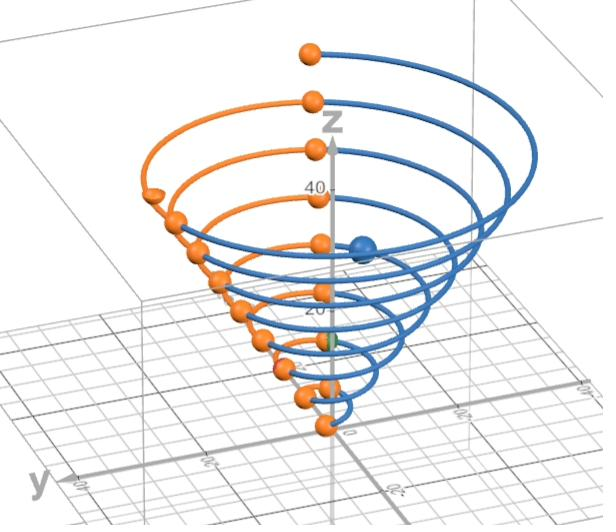
\includegraphics[width=0.72\textwidth]{bilder/kegelhelix}
  \caption{Two superimposed conical helices: the blue curve connects the
    integer points with $n \equiv 1 \pmod{6}$ (major steps,
    $\Delta\theta = 4\pi/3$), and the orange curve connects the points with
    $n \equiv 5 \pmod{6}$ (minor steps, $\Delta\theta = 2\pi/3$).
    The orange spheres mark all integer values $k(n)$ on the helix; both
    primes and composite numbers of the sequence are represented. The
    differing winding densities of the two curves reflect the alternating
    gap--twin pattern of the sequence.}
  \label{fig:conical-helix-twin-gap}
\end{figure}

\section{The Angular Spacing Pattern}

\begin{proposition}[Alternating Pattern]\label{prop:angular-spacing}
The angular spacings between consecutive integer points follow an
alternating pattern:
\begin{align}
\Delta\theta_{\text{major}} &= \theta_{n+4} - \theta_n = \frac{4\pi}{3} \approx 4.189 \quad \text{(for } n \equiv 1 \pmod{6}\text{)}\\
\Delta\theta_{\text{minor}} &= \theta_{n+2} - \theta_n = \frac{2\pi}{3} \approx 2.094 \quad \text{(for } n \equiv 5 \pmod{6}\text{)}
\end{align}
\end{proposition}

\begin{proof}
Direct computation:
\begin{align}
\theta_{n+4} - \theta_n &= \left(\frac{\pi}{3}(n+4) + \frac{\pi}{4}\right) - \left(\frac{\pi}{3}n + \frac{\pi}{4}\right) = \frac{4\pi}{3}\\
\theta_{n+2} - \theta_n &= \left(\frac{\pi}{3}(n+2) + \frac{\pi}{4}\right) - \left(\frac{\pi}{3}n + \frac{\pi}{4}\right) = \frac{2\pi}{3}
\end{align}
\end{proof}

\begin{remark}\label{rem:alternating-pattern}
This alternating pattern of $\frac{4\pi}{3}$ and $\frac{2\pi}{3}$
corresponds geometrically to the alternating ``major steps'' and ``minor
steps'' in the original difference sequence.
\end{remark}

\section{Geometric Corollary: All Primes on the Helix}

We now formulate the central geometric corollary of the preceding
construction.

\begin{theorem}[Primes as a Subset of the Helix]\label{thm:primes-on-helix}
All primes $p > 3$ lie as discrete points on the conical helix at angles
\begin{equation}\label{eq:prime-angles}
\boxed{\theta_p = \frac{\pi}{3}p + \frac{\pi}{4}}
\end{equation}
\end{theorem}

\begin{proof}
The proof is a direct corollary of two known results:

\textbf{Step~1 (Classical number theory, Theorem~\ref{satz:primzahlen}).}
All primes $p > 3$ satisfy $p \equiv 1$ or $5 \pmod{6}$.

\textbf{Step~2 (Geometric construction, Theorem~\ref{thm:integer-points}).}
The helix intersects the plane $z = n$ at the angle
$\theta_n = \frac{\pi}{3}n + \frac{\pi}{4}$ for all
$n \equiv 1, 5 \pmod{6}$.

\textbf{Conclusion.} Since every prime $p > 3$ satisfies the condition
from Step~1, and the helix by Step~2 attains integer heights precisely at
these congruence classes, every prime $p > 3$ lies on the helix at the
angle $\theta_p = \frac{\pi}{3}p + \frac{\pi}{4}$.

\textbf{Important caveat.} The converse does not hold: not every integer
point on the helix corresponds to a prime (see
Section~\ref{sec:composites}).
\end{proof}

\begin{example}[First Primes on the Helix]\label{ex:first-primes}
The first primes greater than 3 and their positions:
\begin{align*}
p = 5 &: \theta_5 = \frac{5\pi}{3} + \frac{\pi}{4} = \frac{23\pi}{12} \approx 6.021\\
p = 7 &: \theta_7 = \frac{7\pi}{3} + \frac{\pi}{4} = \frac{31\pi}{12} \approx 8.117\\
p = 11 &: \theta_{11} = \frac{11\pi}{3} + \frac{\pi}{4} = \frac{47\pi}{12} \approx 12.305\\
p = 13 &: \theta_{13} = \frac{13\pi}{3} + \frac{\pi}{4} = \frac{55\pi}{12} \approx 14.398\\
p = 17 &: \theta_{17} = \frac{17\pi}{3} + \frac{\pi}{4} = \frac{71\pi}{12} \approx 18.587\\
p = 19 &: \theta_{19} = \frac{19\pi}{3} + \frac{\pi}{4} = \frac{79\pi}{12} \approx 20.682\\
p = 23 &: \theta_{23} = \frac{23\pi}{3} + \frac{\pi}{4} = \frac{95\pi}{12} \approx 24.870
\end{align*}
\end{example}

\section{Geometric Interpretation}

\begin{corollary}[Prime Distribution on the Helix]\label{cor:prime-distribution}
The primes greater than 3 form a discrete subset of the helix whose
spacings are determined by the prime gaps in the congruence classes
$1, 5 \pmod{6}$.
\end{corollary}

\begin{remark}[Relation to Prime Gaps]\label{rem:prime-gaps}
If $p$ and $q$ are consecutive primes with $p, q > 3$, the arc length
along the helix between these two points depends on the prime gap $q - p$.

For twin primes ($q = p + 2$):
\[
\Delta\theta = \theta_q - \theta_p = \frac{2\pi}{3}
\]

For cousin primes ($q = p + 4$):
\[
\Delta\theta = \theta_q - \theta_p = \frac{4\pi}{3}
\]
\end{remark}

\section{Composite Numbers on the Helix}\label{sec:composites}

The helix does not contain only primes. Since it geometrically embeds all
indices of the congruence classes $1$ and $5$ modulo~$6$, all composite
numbers belonging to these classes also lie on the curve.

\begin{example}[First Composite Number on the Helix]\label{ex:first-composite}
The first composite number on the helix is $n = 25 = 5^2$:
\[
\theta_{25} = \frac{25\pi}{3} + \frac{\pi}{4} = \frac{103\pi}{12} \approx 26.964
\]
\end{example}

\begin{remark}[Complete Characterisation]\label{rem:complete-characterisation}
The helix contains exactly the set
$\{n \in \mathbb{Z}_{>0} : n \equiv 1, 5 \pmod{6}\}$. The primes $p > 3$
form a distinguished but non-isolable subset therein. The numbers $2$, $3$,
and all $n$ with $n \equiv 0, 2, 3, 4 \pmod{6}$ do not lie on the helix.
\end{remark}

\section{Asymptotic Density}

\begin{proposition}[Density of Primes on the Helix]\label{prop:prime-density}
By the prime number theorem, the density of primes among the integer
points of the helix tends asymptotically to zero:
\[
\lim_{N \to \infty} \frac{\#\{p \leq N : p \text{ prime}, p > 3\}}{\#\{n \leq N : n \equiv 1, 5 \pmod{6}\}} = 0
\]
\end{proposition}

\begin{proof}
The numerator grows as $\sim \frac{N}{\ln N}$ (prime number theorem),
while the denominator grows as $\sim \frac{N}{3}$ (since exactly
$\frac{1}{3}$ of all integers satisfy $n \equiv 1, 5 \pmod{6}$). Hence:
\[
\frac{N/\ln N}{N/3} = \frac{3}{\ln N} \to 0 \quad\text{as } N \to \infty
\]
\end{proof}

\section{Visualisation}

\begin{remark}[Comparison with Other Prime Spirals]\label{rem:comparison-prime-spirals}
In contrast to the Ulam spiral or the Sacks spiral, which represent
empirically discovered patterns, our helix is \emph{derived} from the
arithmetic properties of a specific quadratic sequence. The appearance
of all primes $> 3$ is a \emph{theorem}, not an observation.
\end{remark}

\section{Open Questions}

\begin{enumerate}
\item Can the helix structure yield insights into prime gaps or the
  distribution of twin primes?
\item Is there a natural extension to other congruence-based sequences?
\end{enumerate}
